
\subsection{AEA RCT Registry}
\label{sec:registry}

The \rctr{} (Registry) provides services to the economics (and social science) community at large. Managed at J-PAL and funded by the AEA, registration at the Registry is mandatory for field experiments published in \ac{AER}, \ac{AERI}, \ac{AEJAPP}, and \ac{AEJPOL}, but is also used more broadly in the economics discipline, with numerous publications in top economics journals as well as field journals identifying pre-registration in the Registry. The Registry is available at \href{https://www.socialscienceregistry.org/}{www.socialscienceregistry.org}.\footnote{This section is based in part on information provided by Stuti Goyal, Jack Cavanagh, and Sarah Kopper. All errors are mine.}
%
In collaboration with members of the AEA's \textit{Oversight Committee for Registry of Random Controlled Trials}, the Registry team at J-PAL have continued to work on improving the usability of the Registry, as well as ensuring the availability of Registry data. 


Data for the Registry is being curated and preserved in the \textit{AEA RCT Registry Dataverse} at 
\href{https://dataverse.harvard.edu/dataverse/aearegistry}{dataverse.harvard.edu/dataverse/aearegistry}, allowing for reproducible analysis of the universe of registrations by researchers.%
\footnote{Data shown in this report are derived from \citet{DVN/2RZF2X_2024}, and show data for calendar year \reportyear{}.  
%End-of-year numbers for \reportyear{} were extrapolated based on data from the first 11 months of \reportyear{}, as of \lastday{}. 
} 

% The Data Editor monitors proper reference to and citation of registrations. A registration should be cited in the text and the title footnote as, for example, ``\textit{Zhang (2017)}'' (the title footnote should also mention ``\textit{AEARCTR-0000005}''), and the references should have the appropriate entry:

% \begin{quote}\footnotesize
%     Zhang, Kelly. 2017. "Voter Pessimism and Electoral Accountability: Experimental Evidence from Kenya." AEA RCT Registry. May 02. https://doi.org/10.1257/rct.5-8.0.
% \end{quote}

%{\color{red}Additional data to come.}

%While the AEA journals mentioned above remain among the few economics journals that strictly require registration, 
Usage of the registration continues to increase strongly. As Figures~\ref{fig:registry1} and~\ref{fig:registry2} show, the rate of registrations per year continues to rise, and the registry now has over \regscumul{} registrations, which are being added at a rate of \regsyearly{} per year.  More than \registeredusers{} unique researchers are associated with these registrations (left panel, Figure~\ref{fig:registry2}), \activeusers{} of which are associated with registrations that have been active in \reportyear{}. The share of pre-registrations, favored by some, surpassed post-registrations for the first time in 2021, and remains higher (right panel, Figure~\ref{fig:registry2}). 

% src=https://github.com/J-PAL/AEA_registryanalysis/archive/refs/heads/main.zip

\begin{figure}
\centering
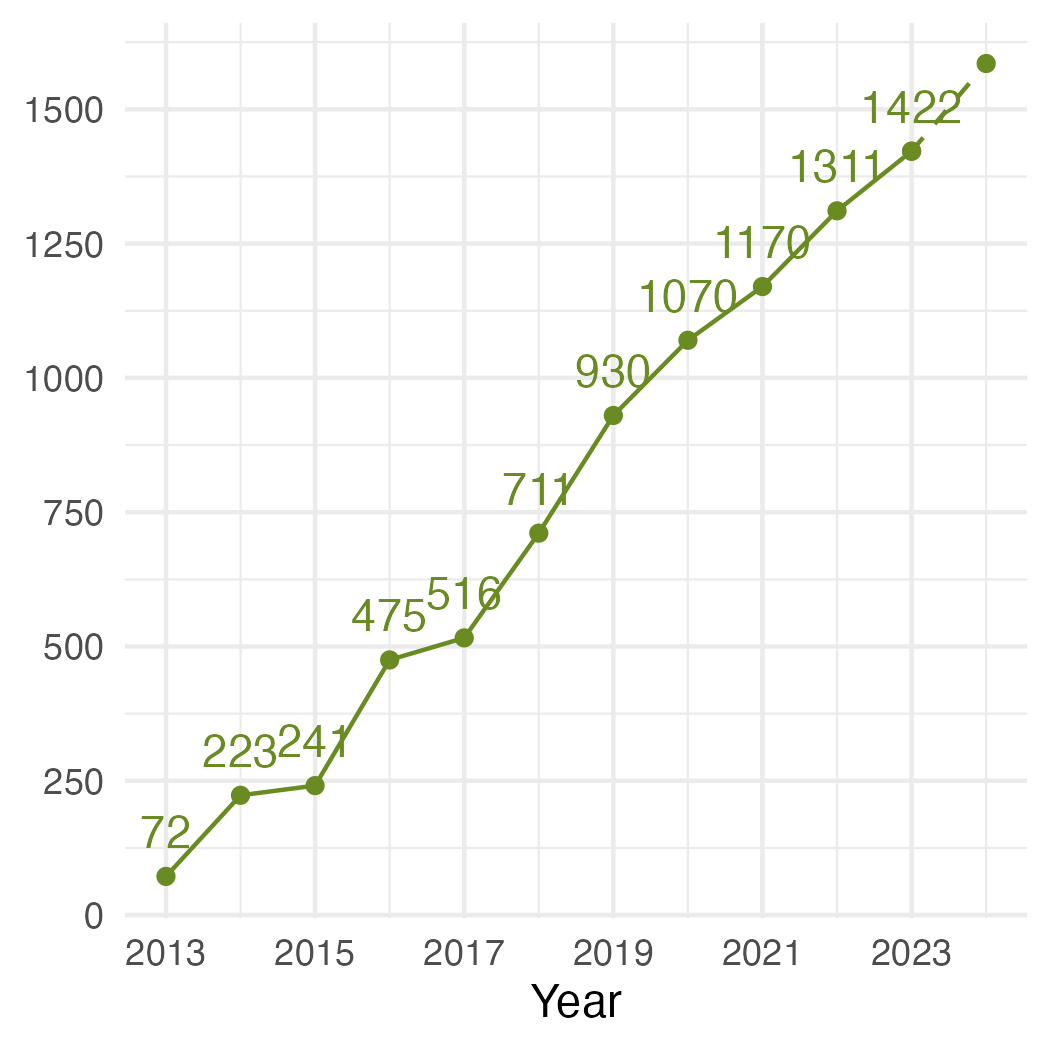
\includegraphics[width=0.4\textwidth]{data/registry/Output/reg_pre_year_2023.png}
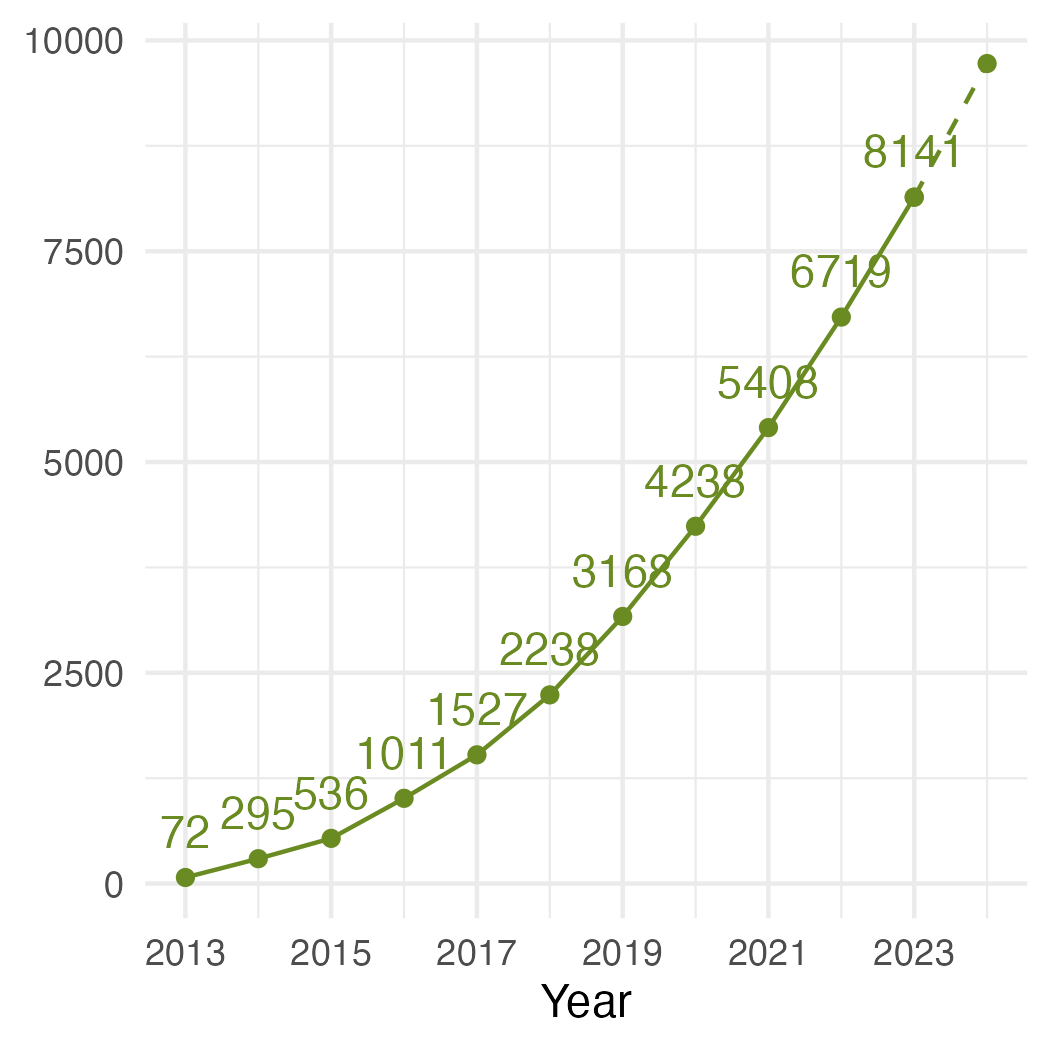
\includegraphics[width=0.4\textwidth]{data/registry/Output/reg_cumulative_2023.png}
\caption{Annual (left) and Cumulative Registrations (right) }
    \label{fig:registry1}
\caption*{\footnotesize Source: \citet{DVN/2RZF2X_2024}. Dashed lines are extrapolated increases for 2024.}
\end{figure}

\begin{figure}
\centering
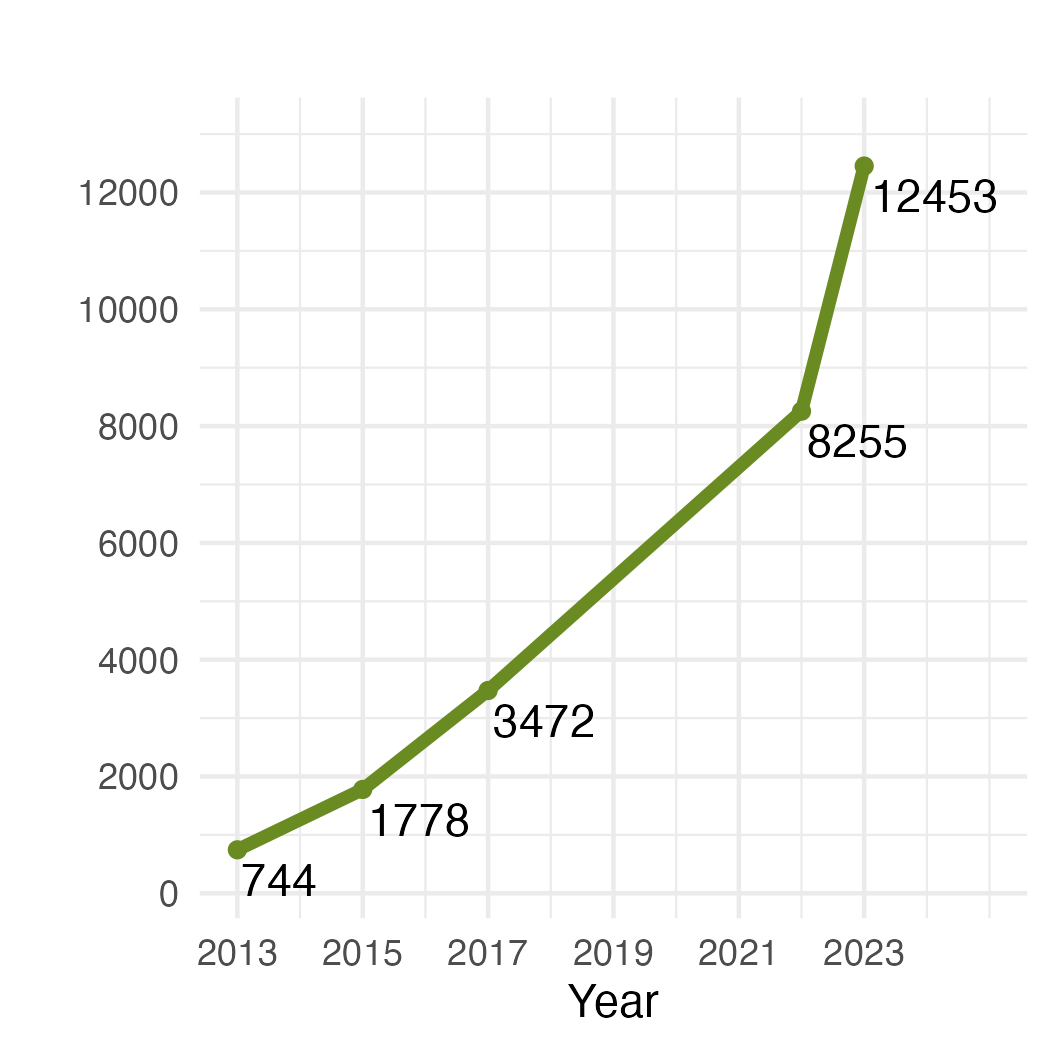
\includegraphics[width=0.4\textwidth]{data/registry/Output/registered_users_2023.png}
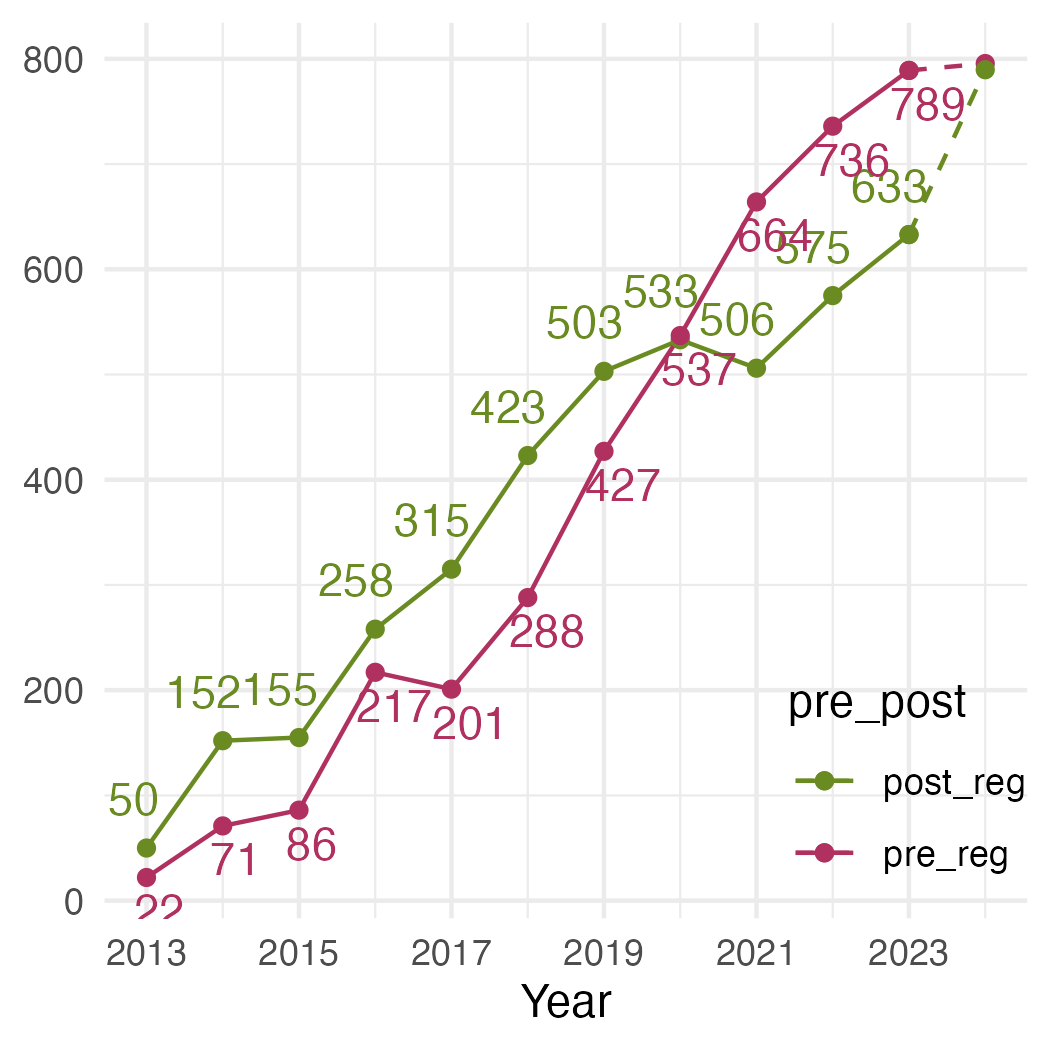
\includegraphics[width=0.4\textwidth]{data/registry/Output/post_pre_reg_2023.png}
\caption{Unique registered investigators (left), Post vs Pre-registrations (right)}
    \label{fig:registry2}
\caption*{\footnotesize Source: \citet{DVN/2RZF2X_2024}. Dashed lines are extrapolated increases for 2024.}
\end{figure}

As the registry has continued to grow, attract new users, and become a standard for experiments across economics and related social sciences, it is improving in its function as a central database of those experiments. In the last five years, an increasing number of articles  use the publicly available registry metadata as either their main analysis data or as a supplement to it. These can be grouped into a few broad sets.  
%
% In particular, multiple published articles and working papers use the Registry to analyze the scientific aspects of (pre-)registration, see \citet{corduneanu-huci_what_2022,
% miguel_evidence_2021,
% murtagh-white_learning_2023,
% leight_publication_2022,
% christensen_open_2019,
% ofosu_pre-analysis_2019,
% laitin_reporting_2021,
% abrams_research_2020,
% corduneanu-huci_politics_2021,
% buckley_role_2022,
% christensen_transparency_2018}.
%
%
One group of papers use the registry to study research transparency questions in the social sciences, either studying the registry as a transparency object in itself \citep{christensen_transparency_2018,abrams_research_2020,miguel_evidence_2021}, taking it as a means to glean information on other transparency behaviors \citep{ofosu_pre-analysis_2019,laitin_reporting_2021}, or  using it as an auditing tool, both for self-reported data \citep{christensen_open_2019} and the implementation of transparency policies \citep{buckley_role_2022}. A second group use the registry data as a significant portion of a larger compiled dataset attempting to proxy for the universe of experiments and experimenters in a particular subset of social science research \citep{corduneanu-huci_politics_2021,corduneanu-huci_what_2022}. A last group of studies use the data to answer meta-scientific questions about the studies on the registry \citep{leight_publication_2022,murtagh-white_learning_2023}.
